\section{Introduction}
\label{sec:intro}

An appealing image may omit a requested object. A fluent summary may remove a
qualification that changes the source's meaning. A research proposal may offer an
interesting hypothesis without an experiment capable of testing it. These are
evaluation problems in open-ended generation: multiple outputs are reasonable,
quality has several dimensions, and no single deterministic verifier defines the
complete ordering. Existing metrics and model-based judges provide useful but
different evidence about that ordering
\citep{fabbri2021summeval,xu2023imagereward,ghosh2023geneval,liu2023geval}.

The availability of more evaluators does not by itself specify how to resolve
their disagreement. A learned metric and a language-model judge may assess
different constructs, or share a blind spot despite producing different scores.
Human feedback is valuable where such evidence is insufficient, but an overall
preference alone does not locate a failure in observation, criteria, reasoning,
or aggregation. Work on model-based judging and human-authored criteria motivates
making these distinctions explicit \citep{zheng2023judging,shankar2024evalgen}.
The resulting research problem concerns both \emph{where to request feedback}
and \emph{how to use it to change an evaluation system}.

We introduce \PtwoE{}, Preference-Guided Evaluator Evolution, for domains with
open-ended outputs and an existing evaluation ecosystem.
Figure~\ref{fig:overview} presents the complete framework. \PtwoE{} maps available
signals to quality dimensions before exposing human labels, mines informative
disagreements, and collects feedback at a declared level of granularity.
An adaptation evidence table connects these judgments to source artifacts and
execution traces. Within P2E, we instantiate evaluator adaptation with
\ERA{} (Evidence-Guided Revision of Agentic Evaluators), a method for revising
executable evaluation programs.

\begin{figure}[t]
\centering
\begin{tikzpicture}[line cap=round,line join=round]
  \path[use as bounding box] (0,0) rectangle (13.7,8.1);
  \node[pTitle,anchor=west] at (0,7.94) {(a) Open-ended generation: four families, domain-specific standards};
  \node[inner sep=0pt,anchor=north] at (6.85,7.69)
    {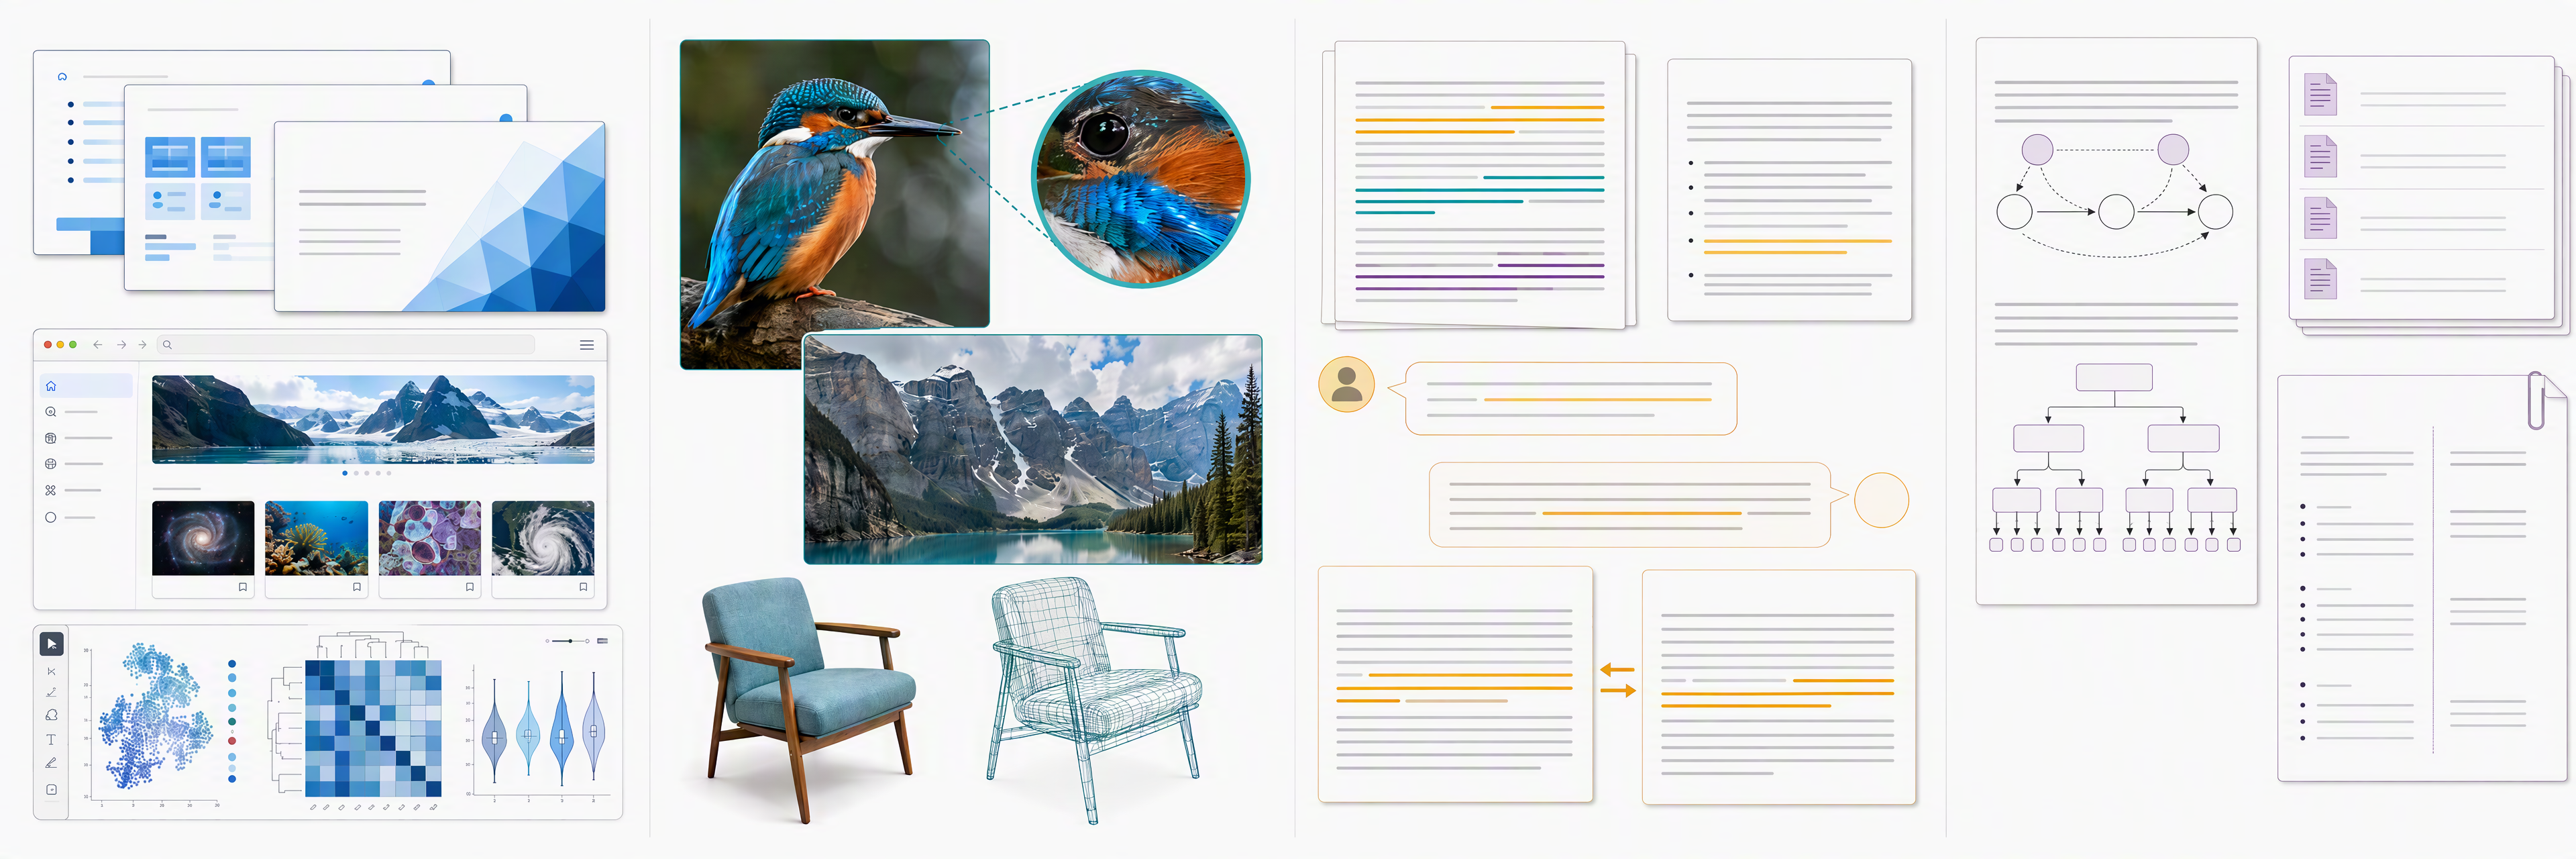
\includegraphics[width=13.65cm]{output/imagegen/domain-panorama-final.png}};
  \foreach \x/\label/\col in {
    1.7125/Structured visuals/pBlue,
    5.1375/Images and 3D/pTeal,
    8.5625/Text generation/pGold,
    11.9875/Automated research/pPlum}{
    \node[pTitle,text=\col,align=center] at (\x,3.04) {\label};
    \draw[draw=\col,line width=1.1pt] (\x-1.5,2.81) -- (\x+1.5,2.81);
  }
  \node[pTitle,anchor=west] at (0,2.48) {(b) Preference mining};
  \node[pTitle,anchor=west] at (5.35,2.48) {(c) Evaluator evolution};
  \node[pTitle,anchor=west] at (10.85,2.48) {(d) Independent uses};

  \node[pCard,fill=pBlue!6,text width=1.35cm,minimum height=.82cm,align=center]
    (space) at (.83,1.77) {Semantic\\space};
  \node[pCard,fill=pGold!7,text width=1.35cm,minimum height=.82cm,align=center]
    (conflict) at (2.6,1.77) {Conflict\\pool};
  \node[pCard,fill=pTeal!7,text width=1.35cm,minimum height=.82cm,align=center]
    (human) at (4.37,1.77) {Human\\feedback};
  \draw[pArrow] (space) -- (conflict);
  \draw[pArrow] (conflict) -- (human);
  \node[pSmall,align=center] at (2.60,1.00)
    {$H_0$ overall \quad $H_1$ dimensional};
  \node[pSmall,align=center] at (2.60,.61)
    {$H_2$ localized \quad $H_3$ rationale};
  \node[pSmall,align=center] at (2.60,.20)
    {Label-blind pool selection};

  \node[pCard,fill=pTeal!7,text width=1.23cm,minimum height=.82cm,align=center]
    (z) at (5.98,1.77) {Evidence\\table $Z$};
  \node[circle,draw=pBlue,fill=pBlue!6,line width=.9pt,
    minimum size=1.35cm,inner sep=1pt,pTitle,align=center]
    (era) at (8.0,1.77) {ERA\\revision};
  \draw[-{Latex[length=1.5mm]},pBlue,line width=.8pt]
    (8.0,2.37) arc[start angle=90,end angle=405,radius=.60cm];
  \node[pCard,fill=pBlue!7,text width=.85cm,minimum height=.82cm,align=center]
    (program) at (9.87,1.77) {Frozen\\$E^*$};
  \draw[pArrow] (human.east) -- (z.west);
  \draw[pArrow] (z) -- (era);
  \draw[pArrow] (era) -- (program);
  \node[pSmall,align=center] at (8.0,.84)
    {Views $A$ \quad Rubrics $K$ \quad Modules $V$\\
     Tools $T$ \quad Routing $\Pi$ \quad Fusion $G$};
  \node[pSmall,align=center] at (8.0,.20)
    {Fixed model; pointwise deployment};

  \foreach \y/\head/\desc/\col in {
    2.00/C1/Alignment and selection/pBlue,
    1.27/C2/Critic-guided refinement/pTeal,
    .54/C3/Reward training: planned/pPlum}{
    \fill[\col!9,rounded corners=2pt] (10.92,\y-.29) rectangle (13.7,\y+.29);
    \node[pTitle,text=\col,anchor=west] at (11.02,\y+.09) {\head};
    \node[pSmall,anchor=west,text=pInk,text width=1.97cm] at (11.61,\y) {\desc};
  }
  \draw[pSoftArrow] (program.east) -- (10.63,1.77) -- (10.63,2.0) -- (10.92,2.0);
  \draw[pSoftArrow] (10.63,1.77) -- (10.63,1.27) -- (10.92,1.27);
  \draw[pSoftArrow] (10.63,1.27) -- (10.63,.54) -- (10.92,.54);
\end{tikzpicture}

\caption{\PtwoE{} connects domain-specific evaluation to human feedback,
evaluator evolution, and independent assessment. (a) Four artifact families.
(b) Disagreement and structured human evidence. (c) \ERA{} revises a six-component
program with a fixed base model. (d) C1 selection, C2 refinement, and planned
C3 reward training. Artifacts, preferences, and feedback are constructed
illustrations; the photograph is generated with GPT Image 2. Arrows denote
information flow, not measured improvements.}
\label{fig:overview}
\end{figure}

Two hypotheses motivate the design. First, disagreements between reliable,
nonredundant signals may make a fixed annotation budget more informative than
uniform sampling. Second, failures that depend on acquiring, routing, and
interpreting evidence may require connected program revisions. A failed
implementation is therefore insufficient to reject its underlying hypothesis.
These expectations call for matched-budget comparisons, not an assumption that
more feedback detail or a larger search space must help.

The research scope extends across structured visual artifacts, image generation
and understanding, text generation, and automated research. A common procedure
is instantiated separately for each evaluation standard. Its value is tested at
three distinct levels: agreement and selection on fixed candidates (C1), changes
to outputs through a frozen critic (C2), and changes to a generator through a
frozen reward (C3). Success at one level does not establish success at the next.
This paper develops the feedback-mining formulation, the ERA revision procedure,
and the controlled evaluation design for these hypotheses.
